%  article.tex (Version 3.3, released 19 January 2008)
%  Article to demonstrate format for SPIE Proceedings
%  Special instructions are included in this file after the
%  symbol %>>>>
%  Numerous commands are commented out, but included to show how
%  to effect various options, e.g., to print page numbers, etc.
%  This LaTeX source file is composed for LaTeX2e.

%  The following commands have been added in the SPIE class 
%  file (spie.cls) and will not be understood in other classes:
%  \supit{}, \authorinfo{}, \skiplinehalf, \keywords{}
%  The bibliography style file is called spiebib.bst, 
%  which replaces the standard style unstr.bst.  

\documentclass[]{spie}  %>>> use for US letter paper
%%\documentclass[a4paper]{spie}  %>>> use this instead for A4 paper
%%\documentclass[nocompress]{spie}  %>>> to avoid compression of citations
%% \addtolength{\voffset}{9mm}   %>>> moves text field down
%% \renewcommand{\baselinestretch}{1.65}   %>>> 1.65 for double spacing, 1.25 for 1.5 spacing 
%  The following command loads a graphics package to include images 
%  in the document. It may be necessary to specify a DVI driver option,
%  e.g., [dvips], but that may be inappropriate for some LaTeX 
%  installations. 
\usepackage{graphicx}
\usepackage{subfig}

\title{Texture mapping 3D planar models of indoor environments with noisy camera poses} 

%>>>> The author is responsible for formatting the 
%  author list and their institutions.  Use  \skiplinehalf 
%  to separate author list from addresses and between each address.
%  The correspondence between each author and his/her address
%  can be indicated with a superscript in italics, 
%  which is easily obtained with \supit{}.

\author{Peter Cheng, Michael Anderson, Stewart He, Avideh Zakhor
\skiplinehalf
University of California, Berkeley\\
}

 

%%%%%%%%%%%%%%%%%%%%%%%%%%%%%%%%%%%%%%%%%%%%%%%%%%%%%%%%%%%%% 
%>>>> uncomment following for page numbers
% \pagestyle{plain}    
%>>>> uncomment following to start page numbering at 301 
%\setcounter{page}{301} 
 
\begin{document}
\maketitle

%%%%%%%%%%%%%%%%%%%%%%%%%%%%%%%%%%%%%%%%%%%%%%%%%%%%%%%%%%%%% 
\begin{abstract}
  Automated 3D modeling of building interiors is used in applications
  such as virtual reality and environment mapping. Texturing these
  models allows for photorealistic visualizations of the data
  collected by such modeling systems. Camera poses obtained by these
  systems often suffer from inaccuracies, resulting in visible
  discontinuities when successive images are projected adjacently onto
  a surface for texturing. Existing methods to stitch images together
  are often computationally expensive and work independently of pose
  estimates and geometry information. We propose a method to refine
  camera poses using both existing estimates and geometry information,
  followed by two different methods to composite images together,
  based on the uniformity of available images. The effectiveness of
  our methods is demonstrated on a number of different indoor
  environments.
\end{abstract}

% >>>> Include a list of keywords after the abstract

\keywords{Texture Mapping, Reconstruction, Image Stitching, Mosaicing}

%%%%%%%%%%%%%%%%%%%%%%%%%%%%%%%%%%%%%%%%%%%%%%%%%%%%%%%%%%%%%
\section{Introduction}
\label{sec:introduction} % \label{} allows reference to this section
Three-dimensional modeling of indoor environments has a variety of
applications such as training and simulation for disaster management,
virtual heritage conservation, and mapping of hazardous sites. Manual
construction of these digital models can be time-consuming, and as a
result, automated 3D site modeling has garnered much interest in
recent years. CITATION

The first step in automated 3D modeling is the physical scanning of an
environment's geometry. An indoor modeling system must recover its own
poses within an environment while simultaneously reconstructing the 3D
structure of the environment itself. CITATION. This is known as the
simultaneous localization and mapping (SLAM) problem, and is generally
solved by taking readings from laser range scanners, cameras, and
inertial measurement units (IMUs) at multiple locations within the
environment.

In this paper, we work with data obtained from a backpack-mounted
system, carried by an ambulatory human. Such a system provides
advantages over more common wheel-mounted systems in terms of agility
and portability, but results in much higher localization error and
uncertainty overall. CITATION. As a result, common methods for texture
mapping generally produce poor results, leading to the development of
the approaches contained in this paper. Besides localization
information and images, environment geometry is required as well for
texture mapping. In this paper we work mainly with models obtained by
fitting planar surfaces to point clouds generated by the backpack
system. CITATION. We have also developed an appropriate method to work
with near-planar triangular meshes, as described in APPENDIX
SOMETHING.

Though our texture mapping procedure was designed with the
aforementioned system in mind, it is easily generalizable to any other
system, provided the required inputs of planar geometry, images with
rough extrinsic pose estimates, and either known or estimated
intrinsic camera calibration matrices. An important benefit of our
method is its relatively low complexity and modularity of each step,
allowing for quick tuning of parameters and easy accomodation of new
input data given updates in localization or model-generation
algorithms.

The remainder of the paper is organized as follows. Section X explains
how input images are projected onto our geometry and simple approaches
towards texturing. Section X covers more sophisticated existing
approaches to image matching and stitching, and their performance on
our datasets. Section X contains our approach towards image alignment,
followed by Section X, which describes compositing approaches. Section
X contains further results and conclusions, as well as areas for
future work.
%%%%%%%%%%%%%%%%%%%%%%%%%%%%%%%%%%%%%%%%%%%%%%%%%%%%%%%%%%%%%

\section{Simple Texture Mapping}
\label{sec:simpleTextureMapping}
\begin{figure}
  \centering
  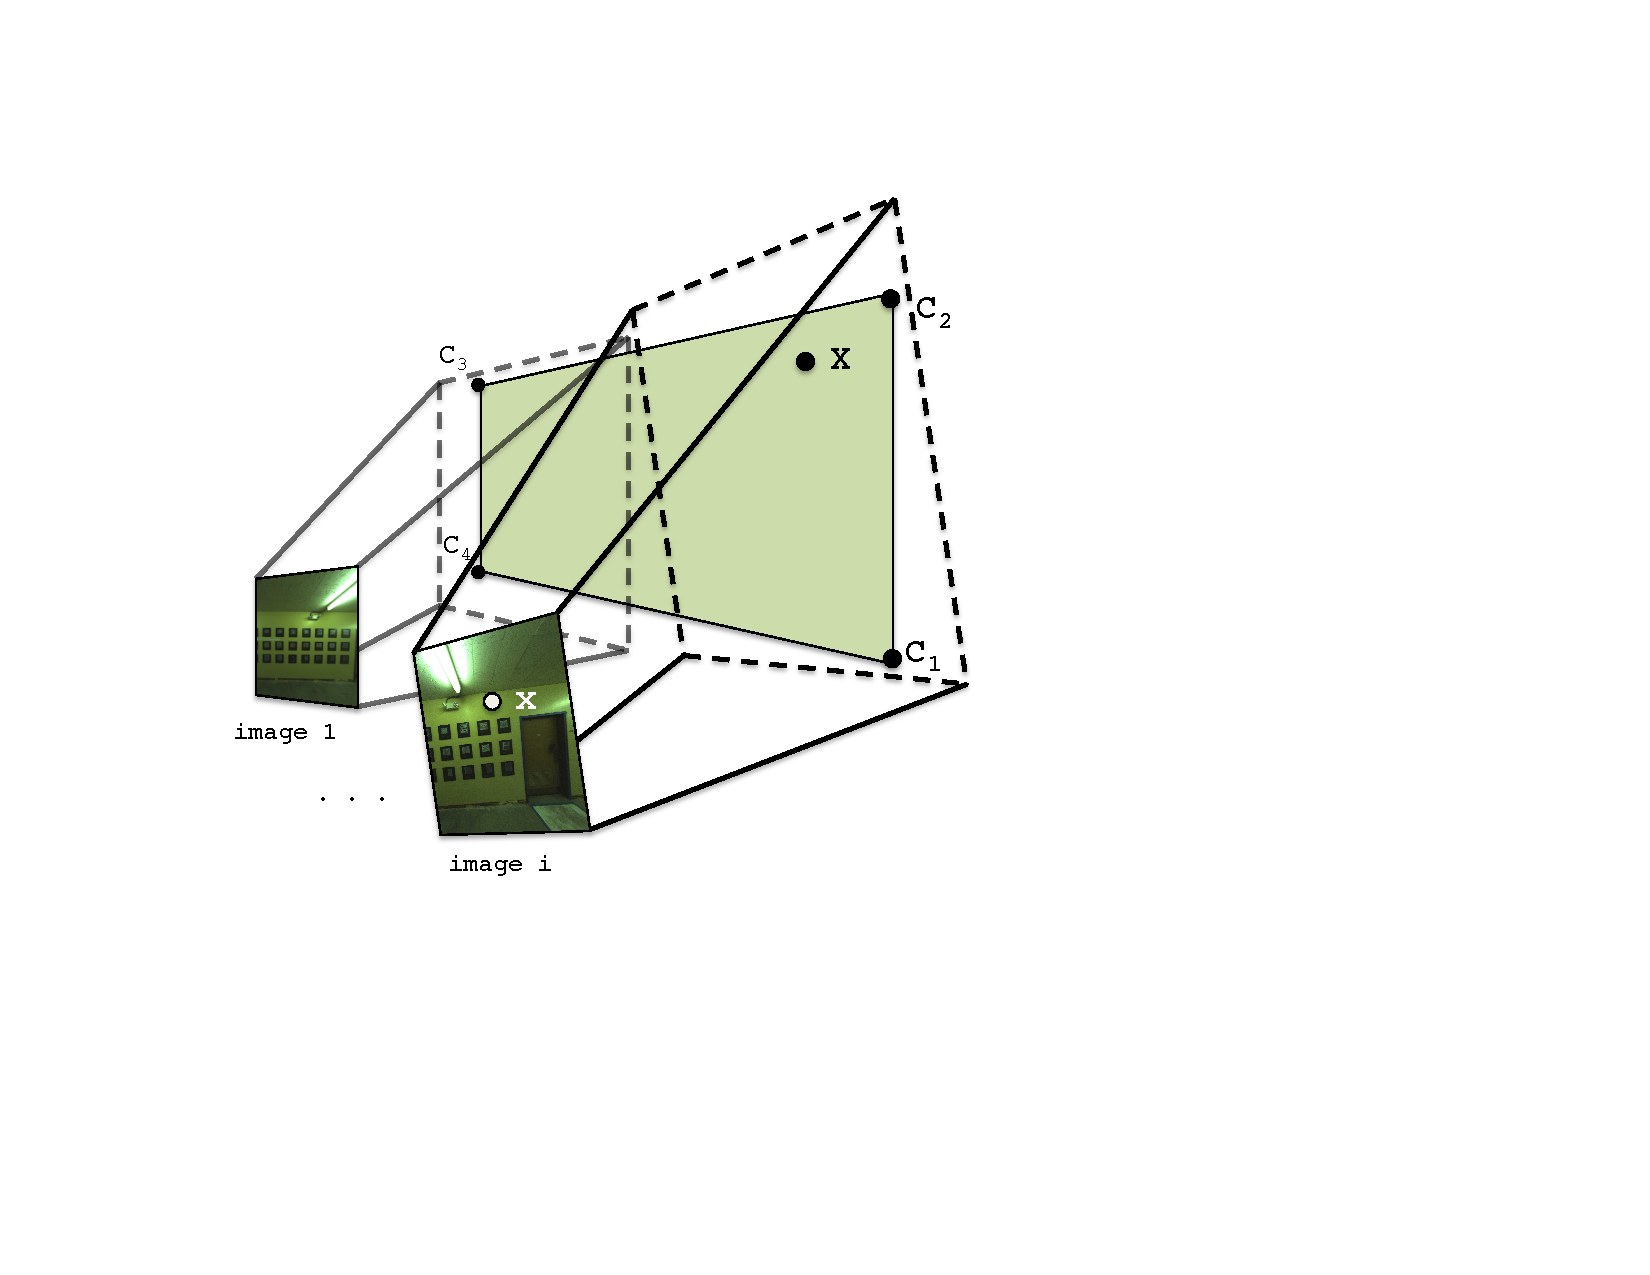
\includegraphics[height=2in]{Projection.pdf}
  \caption{Planes are specified in 3D space by four corners $C_1$ to
    $C_4$. Images are related to each plane through the camera matrics
    $P_{1..m}$. }
  \label{fig:projection}
\end{figure}

The geometry of the texture mapping process for a plane is shown in
Figure \ref{fig:projection}.  As described earlier, we are provided
with a set of $M$ images to texture the target plane. Each image has a
camera matrix $P_i$ for $i=1..M$, which translates a 3D point in the
world coordinate system to a 2D point or pixel in image $i$'s
coordinates. A camera matrix $P_i$ is composed of the camera's
intrinsic parameters, such as focal length and image center, as well
as extrinsic parameters which specify the rotation and translation of
the camera's position in 3D world coordinates at the time that image
$i$ is taken. These extrinsic parameters are determined by the
backpack hardware and localization algorithms \cite{chen2010indoor,
  liu2010indoor, kua2012loopclosure} and are quite noisy.

Because our backpack system takes photos at a rate of 5 Hz, thousands
of images are available for texturing each surface in our model. Our
goal in designing a texture mapping process is to decide which of
these images should be used, and where their contents should map onto
the texture, in order to minimize any visual discontinuities or seams
that would suggest that the plane's final texture is not composed of a
single continuous image.

Ignoring the fact that the camera matrices $P_{1..M}$ are inaccurate,
we can texture the plane by discretizing it into small square tiles,
in our case 5 pixels across, and choosing an image to texture each
tile.

We choose to work with rectangular units to ensure that borders
between any two distinct images in the final texture are either
horizontal or vertical. Since most strong environmental features
inside buildings are horizontal or vertical, any visible seams in our
texture intersect them minimally and are less noticeable.

In order to select an image for texturing a tile $t$, we must first
gather a list of candidate images that contain all four of its
corners, which we can quickly check by projecting $t$ into each image
using the $P_i$ camera matrices. Furthermore, each candidate image
must have been taken at a time when its camera had a clear
line-of-sight to $t$, which can be calculated using standard
ray-polygon intersection tests between the camera location, $t$, and
every other plane \cite{rayintersection}.

Once we have a list of candidate images for $t$, we define a scoring
function in order to objectively select the best image for texturing
$t$. Since camera pose errors compound over distance, we wish to
minimize the distance between cameras and the surfaces they
texture. Additionally, we desire images that are projected
perpendicularly onto the plane, maximizing the resolution and amount
of useful texture available in their projections, as well as
minimizing any parallax effects due to real-world geometry not
accurately represented by our digital model. In other words, we wish
to minimize the angle between the tile's normal vector and the camera
axis for images selected for texture mapping. These two criteria can
be met by maximizing the function $\frac{1}{d} (-1 \cdot \vec{c})
\cdot \vec{n}$ as shown in Figure
\ref{fig:scoringFunction}. Specifically, $d$ is the distance between
the centers of a camera and a tile, and $\vec{n}$ and $\vec{c}$ are
the directions of the plane's normal and the camera axis respectively.

\begin{figure}
  \centering
  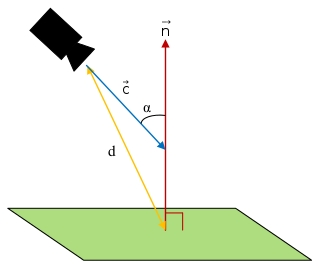
\includegraphics[height=1.5in]{scoringFunction.jpg}
  \caption{We minimize camera angle $\alpha$ and distance $d$ by
    maximizing the scoring function $\frac{1}{d} (-1 \cdot \vec{c})
    \cdot \vec{n}$}
  \label{fig:scoringFunction}
\end{figure}



\begin{figure}[h!]
  \centering \subfloat[][]{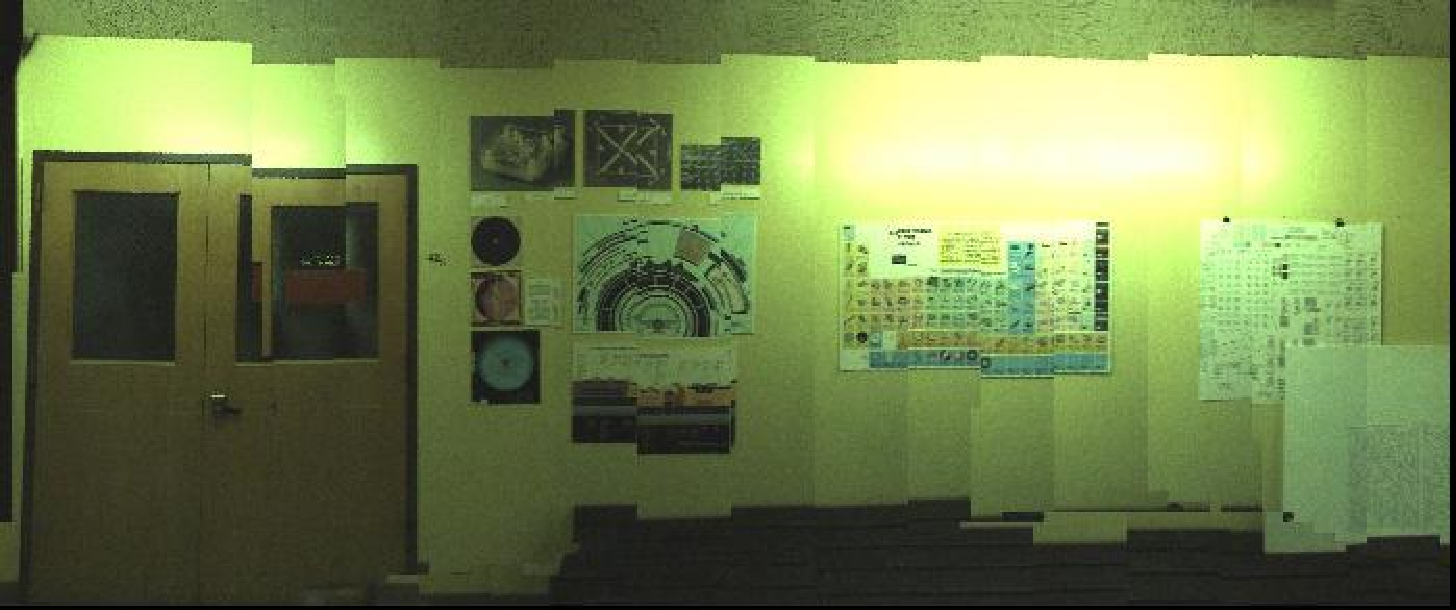
\includegraphics[width=3in,
    height=0.97in]{wall2_naive.pdf}}

  \centering \subfloat[][]{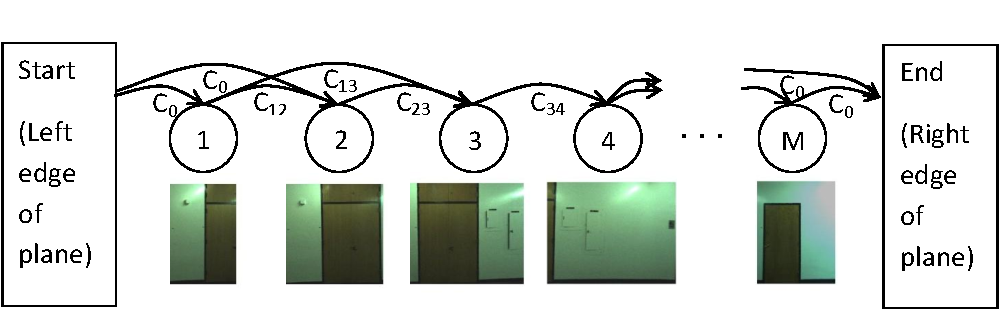
\includegraphics[width=3in,
    height=0.97in]{wall2_naive_shift.pdf}}

  \centering \subfloat[][]{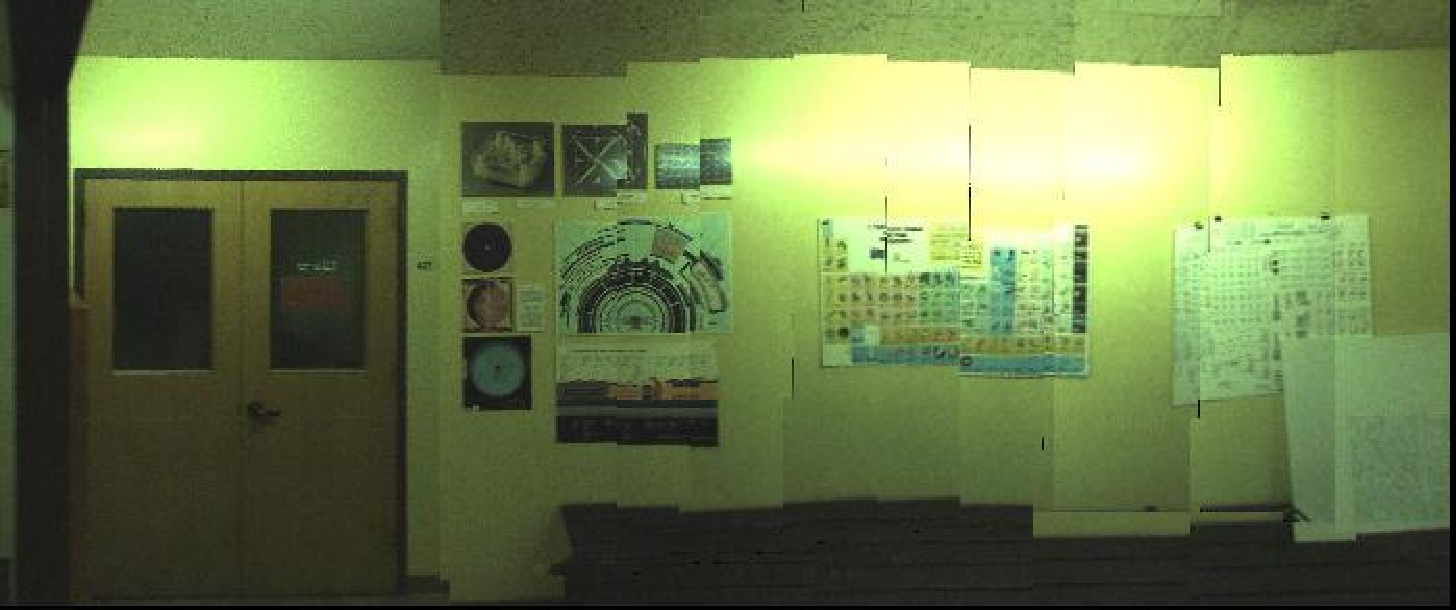
\includegraphics[width=3in,
    height=0.97in]{wall2_cache_shift.pdf}}

  \centering \subfloat[][]{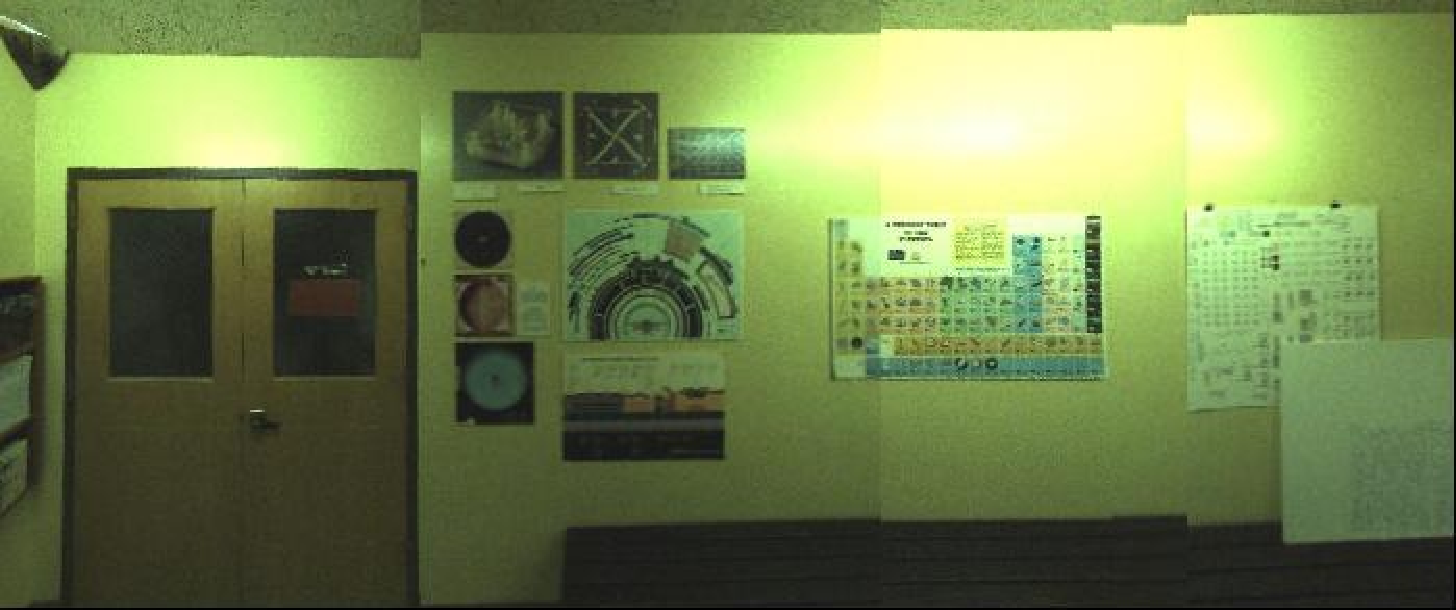
\includegraphics[width=3in,
    height=0.97in]{wall2_shortest_shift.pdf}}

  \centering \subfloat[][]{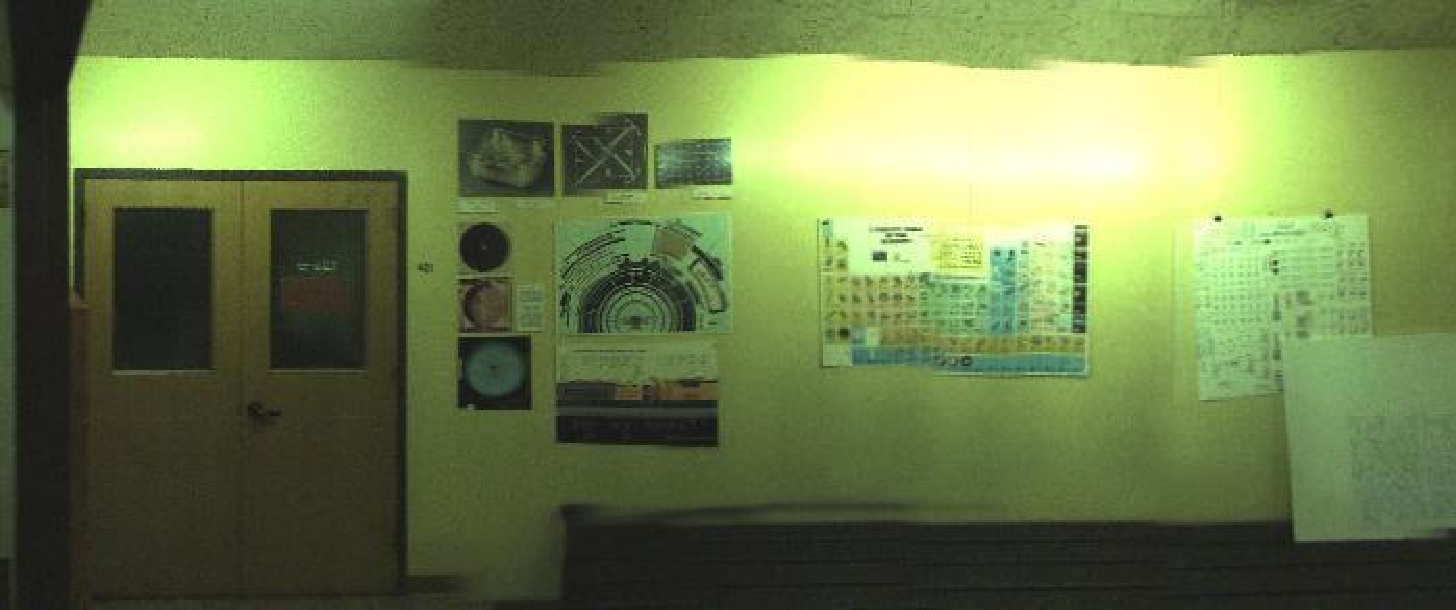
\includegraphics[width=3in,
    height=0.97in]{wall2_cache_shift_blend.pdf}}

  \centering \subfloat[][]{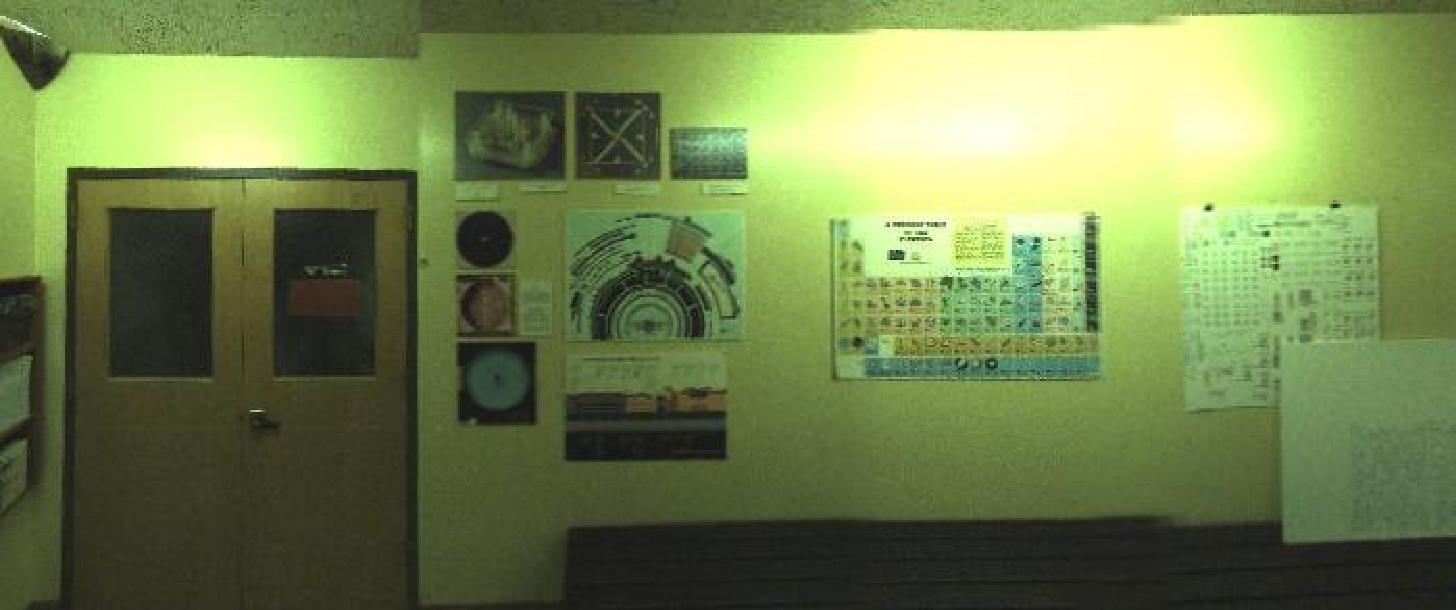
\includegraphics[width=3in,
    height=0.97in]{wall2_shortest_shift_blend.pdf}}
  \caption{(a) Simple mapping. (b) Simple mapping after image
    alignment. (c) Mapping with caching after image alignment. (d)
    Shortest path texturing after image alignment). (e) same as (c)
    with blending. (f) same as (d) with blending.}
  \label{fig:compareAll}
\end{figure}


As Figure \ref{fig:compareAll}(a) demonstrates, this approach leads to
the best texture for each tile independently, but results in many
image boundaries with abrupt discontinuities between tiles, due to
significant misalignment between images. Given our high number of
input images, it makese sense to further refine the image selection
procedure, as performed in Section \ref{sec:imageCompositing}, but for
our solution to be more robust, we first perform image alignment in
order maximize the accuracy of each image.

\section{Existing Approaches to Image Alignment}
\label{sec:existingApproaches}
Stitching together multiple images to produce a larger image is a
commonly performed task, with many successful approaches over the past
few decades. Parts of images are first matched to eachother, through
direct pixel comparisons, or more commonly through feature detection
and matching. Images are then adjusted to maximize matches, either by
calculating homographies between pairs of images, or by
modifying camera poses in 1 to 6 degrees of freedom.

Feature detection and matching works best when multiple unique visual
references exist in the environment and are present within multiple
images. In contrast, our indoor environments have a high
prevalence of bare surfaces, as well as repeating textures that cause
difficulty in disambiguating features. This lack of strong reference
points results in high uncertainty when matching images together.

Additionally, our datasets often contain long chains of images, which
leads to error accumulation when image correspondences are not
accurate. For example, when matching a long chain of images through
homographies, a pixel in the $nth$ image must be translated into the
first image's coordinates by multiplying by the $3\times3$ matrix $H_1
H_2 H_3 ... H_n$. Any error in one of these homography matrices is
propagated to all further images, resulting in drift. Figure
\ref{fig:mosaic3D}(b) shows the output of the AutoStitch software
package, which performs homography-based image mosaicing
\cite{autostitch}. Even with many features spread across this surface,
the mosaicing produces errors that cause straight lines to appear distorted, despite the fact that it was generated after careful hand
tuning. Many areas with fewer visual features simply failed outright
using this approach.

\begin{figure}
  \centering
  \subfloat[][]{
\includegraphics[width=3in]{Graph_crop.pdf}}

  \centering
  \subfloat[][]{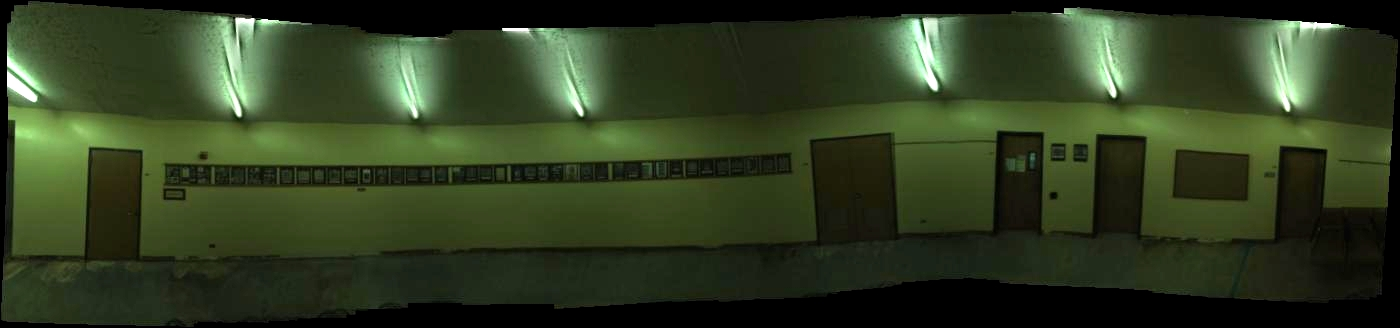
\includegraphics[width=3in]{panoMy.jpg}}
  \caption{Texture alignment via (a) the graph-based localization
    refinement algorithm from \cite{chen2010indoor} and (b) image
    mosaicing.}
  \label{fig:mosaic3D}
\end{figure}

Image projections can also be aligned by iteratively adjusting camera
poses to maximize matches. This is generally done over 6 degrees of
freedom. CITATION. Applying the approach in the LIU2010INDOOR paper
however, results again in error accumulation and drift as shown in
Figure \ref{fig:mosaic3D}(a). Furthermore, such nonlinear optimization
approaches IS IT? BETTER CHECK have high complexity and runtime, and the
entire solution must be recomputed given any changes in input data.


\section{2D Image Alignment with Geometry Information}
\label{sec:2dAlignment}
In this section, we describe our method of efficient and robust image
alignment. Our approach consists of four parts. First, all images are
projected onto the surface and rotated such that detected lines within
them are parallel to lines comprising the surface's boundary and
intersection with other surfaces. Next, these projections are shifted
such that interior lines near surface intersections are matched
up. Following this, occlusion checks are performed to remove invalid
parts of each image for the target surface. These first three steps
are all image-independent and are performed in parallel. Finally, we
detect SIFT feature matches between pairs of images and solve a linear
least squares problem in 2D to maximize matches.

All of our calculations and alignments are performed in 2D, partly for
efficiency, and partly because the nature of our input data is such
that the majority of localization error is 2D, in the same plane as
the surface being projected onto. Recall that our data acquisition
system is backpack-mounted, with cameras facing to the sides of the
operator. The operator attempts to walk parallel to walls, and the
localization and model-generation algorithms that provide our input
can conform the operator's path to be straight and parallel to
detected surfaces. Since the operator walks as upright as possible,
errors in roll and yaw, as well as the operator's distance from
parallel surfaces are minimal. Thus, our highest errors stem from
uncertainty in the operator's pitch, equivalent to rotation around the
camera axes, as well as location along surfaces. These equate to 2D
rotation and translation in a surface's plane.

\subsection{Geometry-based Alignment}
\label{sec:geometryAlignment}
After computing each image's projection onto the target surface, as
described in Section \ref{sec:simpleTextureMapping}, we detect lines
in the projections using Hough transforms. Experience and intuition
show that walls in indoor environments contain linear features that
are either horizontal or vertical, often corresponding to doors,
windows, posters, etc. Thus, when texturing walls, we rotate images in
2D such that dominant lines are made to be horizontal or
vertical. Though not relevant in our datasets, this can be
extrapolated such that lines are oriented with a wall's boundaries,
for example in areas with a slanted roof.

\begin{figure}
  \centering
  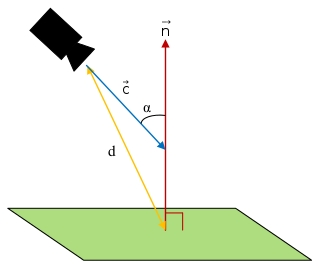
\includegraphics[height=1.5in]{geometryFeature.jpg}
  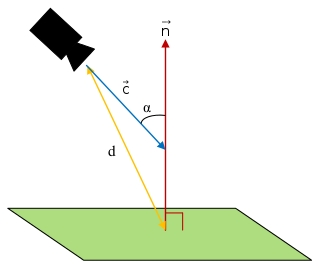
\includegraphics[height=1.5in]{imageCorner.jpg}
  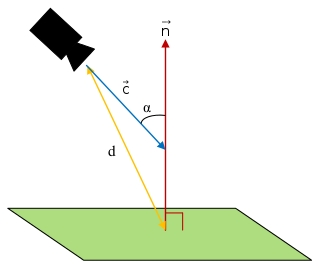
\includegraphics[height=1.5in]{geometryImageAlign.jpg}
  \caption{(a) The red lines indidcate plane intersections that can be used as geometry reference points. (b) A corresponding corner in an image, detected as a line. (c) The image rotated and shifted to align with geometry.}
  \label{fig:geometryAlignment}
\end{figure}


At this point in time, image occlusions have not been accounted
for. As a result, some image projections contain texture that should
project to an adjacent surface, generally with a linear boundary where
the two surfaces meet. If this linear boundary is detected by Hough
transform, the image is rotated and shifted in 2D such that the visual
boundary between two surfaces matches the physical boundary in our
digital model. An example of such an adjustment is in Figure \ref{fig:geometryAlignment}

To perform the rotation and alignment, a robust method would be to
detect all line matches and solve for an optimal homography. In nearly
all cases however, we find that a single 2D rotation is sufficient to
properly align lines in an image. We also rarely have more than one
linear geometry feature to match to. As a result, we do WHATEVER WE DO, and then indicate which images are aligned to geometry, which is useful in Section \ref{sec:robustSIFTFeatureMatching}

\subsection{Image Occlusion}
\label{sec:imageOcclusion}
Now that images have been aligned to geometry where possible, we
perform a simple recursive occlusion procedure on each image. This is
done by performing the intersection tests in section
\ref{sec:simpleTextureMapping} in a regularly spaced grid. Where four
corners of a rectangular region are occluded, texture is
removed. Where no corners are occluded, nothing occurs. Where there is
a mixture of both, the rectangular region is subdivided into four, and
the same process is performed on each. By performing Section
\ref{sec:geometryAlignment}'s alignment procedure before occlusion, we
remove all erroneous texture belonging to other surfaces, which is
necessary for the next section.

\subsection{2D Feature Alignment}
\label{sec:robustSIFTFeatureMatching}
Our next step is to align overlapping images by searching for
corresponding points between all pairs of overlapping images. We use
SIFT features for their high detection rate, and choose to use feature
alignment rather than pixel or intensity-based alignment due to the
differences in lighting as well as possible occlusion among our
images, both of which feature alignment is less sensitive to
\cite{lai1999robust, lowe1999object, mikolajczyk2005performance,
  szeliski2006image}.  In our implementation, we use SiftGPU, by
PERSON CITATION, for both feature detection as well as pairwise
matching. These matches determine $d^x$ and $d^y$ distances between
each pair of features for two image projections, though these
distances may not always be the same for different features. Since
indoor environments often contain repetitive features such as floor
tiles or doors, we need to ensure that SIFT-based distances are
reliable. First, we only perform alignment on pairs of images that
overlap given the original noisy poses. Secondly, we discard feature
matches that correspond to an image distance greater than 40 pixels
from what the noisy poses estimate. In order to utilize the remaining
feature matches robustly, the RANSAC framework
\cite{fischler1981random} is used to estimate the optimal $d^x_{i,j}$
and $d^y_{i,j}$ distances between two images $i$ and $j$. The RANSAC
framework requires a fitting function and a distance function. For
this application, the fitting function simply finds the average
distance between matches in a pair of images. The distance function
for a pair of points is chosen to be the difference between those
points' SIFT match distance and the average distance computed by the
fitting function. We use a 10 pixel outlier threshold, so that SIFT
matches are labeled as outliers if their horizontal or vertical
distances are not within 10 pixels of the average distance computed by
the fitting function.

We now use the calculated $d^x_{i,j}$ and $d^y_{i,j}$ distances
between each pair of images to refine their positions using weighted
linear least squares. Recall that there are a total of $M^{2}$
possible pairs of images, though we only generate distances between
images that overlap at SIFT feature points. Given these distances and
the original image location estimates, we can solve a least squares
problem ($\textrm{min}_{\vec{\beta}} ||A \vec{\beta} -
\vec{\gamma}||_2^2 $) to estimate the location of the images on the
plane. The $M$-dimensional vector $\vec{\beta}$ represents the unknown
$x$ location of each image on the plane for $1 \dots M$. The optimal
$x$ and $y$ locations are obtained in the same way, so we only
consider the $x$ locations here:

\[\vec{\beta} =
\begin{pmatrix}
  x_1, & x_2, & x_3, & \cdots & x_{M-1}, & x_M
\end{pmatrix}
\]

The $N \times (M+1)$ dimensional matrix $A$ is constructed with one
row for each pair of images with measured distances produced by the
SIFT matching stage. A row in the matrix has a $-1$ and $1$ in the
columns corresponding to the two images in the pair. For example, the
matrix below indicates a SIFT-based distance between images 1 and 2,
images 1 and 3, images 2 and 3, etc.
\[
A =
\begin{pmatrix}
  -1 & 1 & 0 & \cdots & 0 & 0\\
  -1 & 0 & 1 & \cdots & 0 & 0\\
  0 & -1 & 1 & \cdots & 0 & 0\\
  \vdots  & \vdots & \vdots & \ddots & \vdots  & \vdots\\
  0 & 0 & 0 & \cdots & 1 & 0 \\
  0 & 0 & 0 & \cdots & -1 & 1 \\
  1 & 0 & 0 & \cdots & 0 & 0 \\
\end{pmatrix}
\]
If only relative distances between images are included, the absolute
location of the images can not be calculated, and the matrix is rank
deficient. From Section \ref{geometryBasedAlignemtn}, a number of
images are anchored to geometry points, and thus their locations can
be used to anchor the rest in place. In case no anchor images exist,
we simply arbitrarily pick an image. In the above matrix, the first
image is set to be such an anchor, simply by placing a $1$ in its
column

The $N$-dimensional observation vector $\vec{\gamma}$ is constructed
using the SIFT-based distances generated in the RANSAC matching
stage. Elements in the observation vector corresponding to anchor
images are simply their locations as determined by the original noisy
localization. Thus $\vec{\gamma}$ can be written as:

\[
\vec{\gamma}^T =
\begin{pmatrix}
  d_{1,2}, &d_{1,3}, &d_{2,3}, &\hdots &d_{N-2,N-1}, &d_{N-1,N}, &x_1
\end{pmatrix}
\]

The $\vec{\beta}$ that minimizes $||A \vec{\beta} -
\vec{\gamma}||_2^2$ results in a set of image locations on the plane
that best honors all the SIFT-based distance measurements between
images. This solution however does not make use of our noisy camera
poses, and will fail when no SIFT matches are found between one
segment of the plane and another. To account for this, we add rows to
the $A$ matrix and observations to the $\vec{\gamma}$ vector
corresponding to the original noisy distances. We then solve a
weighted least squares problem where the SIFT distances and anchor
values are given a high weight e.g. 1, while the noisy distances are
given a smaller weight e.g. 0.01.

After completing this same process for the $y$ dimension as well, and
making the resultant shifts, our images overlap and match each other
with far greater accuracy. Applying the simple mapping scheme in
Section \ref{sec:simpleTextureMapping} results in X, which has far
fewer seams, but can still be improved.

\section{Image Compositing}
\label{sec:imageCompositing}
In this section, we revisit the tile-based texturing approach from
Section \ref{sec:simpleTextureMapping}, with an added caching
mechanism to reduce image boundaries. This method works well given all
manner of camera poses and surfaces, but for cases where we have large
sections of usable texture from images, we propose an alternate method
that further reduces image boundaries.

\subsection{Tile-Mapping with Caching}
\label{sec:mappingWithCaching}
From Section \ref{sec:simpleTextureMapping}, we saw that
discontinuities occur where adjacent tiles are textured by different
images. Though image alignment removes many such discontinuities,
there are still cases where seams are visible due to imprecise
matching or other factors such as lighting differences. To reduce the
cases where this happens, it makes sense to take into account image
selections made by neighboring tiles while texture mapping a given
tile. By using the same image across tile boundaries, we can eliminate
a discontinuity altogether. If this is not possible because a tile is
not visible in images used by neighboring tiles, using similar images
across tile boundaries also leads to less noticeable discontinuities.

Essentially a caching mechanism, we select the best image for a tile
$t$ by searching through two subsets of images for a viable candidate,
before searching through the entire set of valid images. The first
subset of images is the images selected by adjacent tiles that have
already been textured. We must first check which of these images can
map to $t$, and then of those, we make a choice according to the
scoring function in Figure \ref{fig:scoringFunction}. Before reusing
this image, we ensure it meets the criteria $\alpha < 45^\circ$, in
order to ensure a high resolution projection, with $\alpha$ as the
camera angle as shown in Figure \ref{fig:scoringFunction}.

If no satisfactory image is found in the first subset, we check the
second subset of images, consisting of those taken near the ones in
the first subset, both spatially and temporally. These images are not
the same as the ones used for neighboring tiles, but are taken at a
similar location and time, suggesting that their localization and
projection are quite similar, and thus likely matched more
accurately. Again, if no viable image is found according to the same
criteria, we search the entire set of candidate images, selecting
based on the same scoring function from Figure
\ref{fig:scoringFunction}.

The result of this caching approach is shown in Figure X, where seams
are now greatly reduced as compared to Figure X2.

\begin{figure}
  \centering
  \subfloat[][]{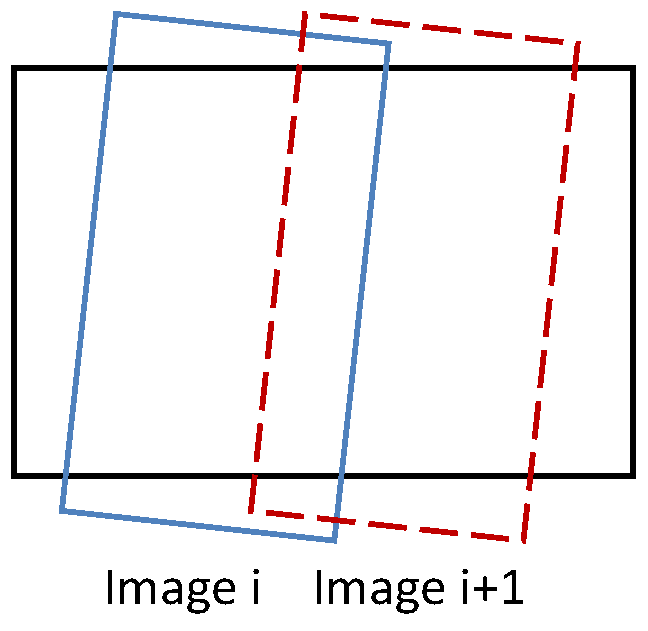
\includegraphics[width=1in]{projectionWall.pdf}}
  \centering
  \subfloat[][]{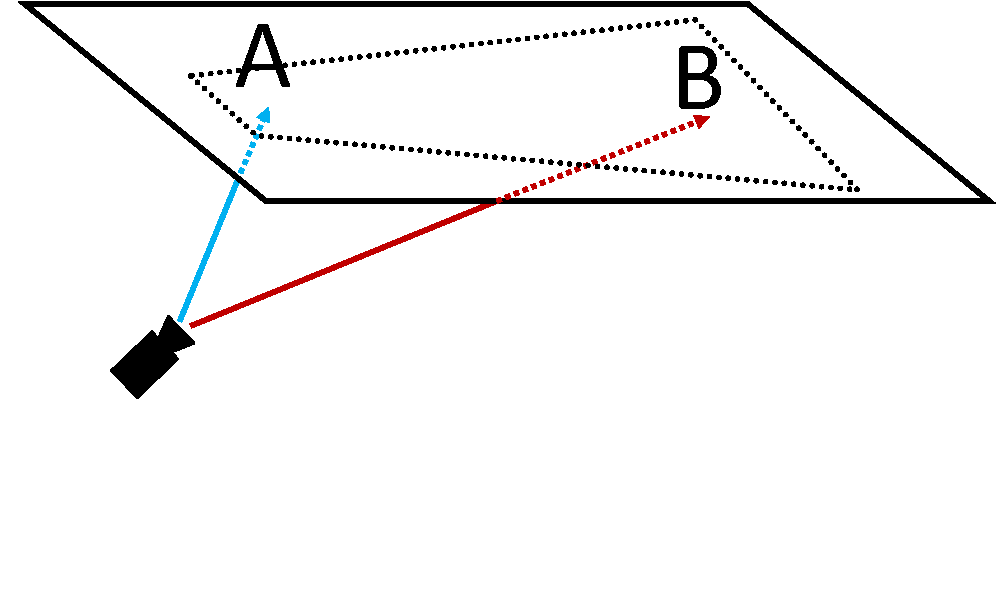
\includegraphics[width=1.1in]{projectionCeiling.pdf}}
  \centering
  \subfloat[][]{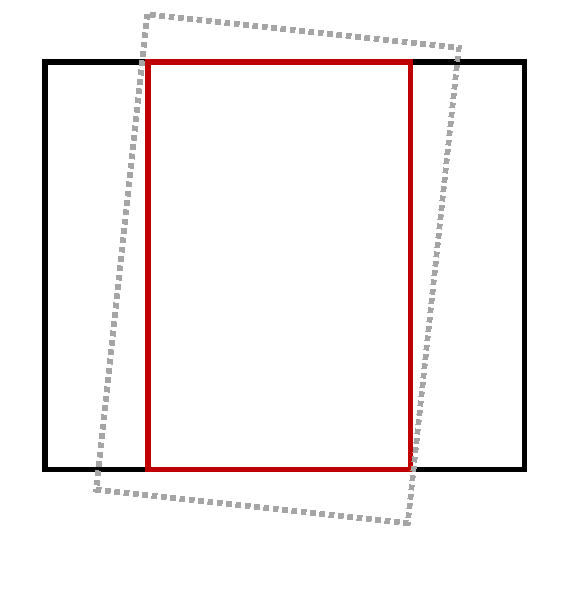
\includegraphics[width=0.9in]{projectionWallCrop.pdf}}
  \caption{(a) Images for vertical planes are tilted, but their
    effective camera axis is more or less normal to the plane. (b) The
    effective camera axis for ceilings is at an angle with respect to
    the plane normal. (c) Wall images are cropped to be rectangular.}
  \label{fig:projectionAngles}
\end{figure}


As mentioned earlier, our data comes from a mobile backpack
system. Human operators can not carry the backpack in a perfectly
upright position and are bent forwards at 15 to 20 degrees with
respect to the vertical direction. As a result, cameras facing
sideways are head on with respect to vertical walls, while cameras
oriented towards the top or bottom of the backpack are at an angle
with respect to horizontal floors and ceilings. This is depicted in
Figures \ref{fig:projectionAngles}(a) and
\ref{fig:projectionAngles}(b). These oblique camera angles for
horizontal surfaces translate into textures that span extremely large
areas once projected, as shown in Figure
\ref{fig:projectionAngles}(b). Using the tile-based texture mapping
criteria from Figure \ref{fig:scoringFunction}, such projections have
highly varying scores depending on the location of a tile on the
plane, as shown again in Figure \ref{fig:projectionAngles}(b). Thus,
the tiling approach in this section is a good choice for texturing
floors and ceilings, as it uses the parts of image projections that
maximize resolution and accuracy for their respective plane locations,
e.g. areas near point A in Figure \ref{fig:projectionAngles}(b), but
not near point B.


\subsection{Shortest Path Texturing}
\label{sec:shortestPath}
For vertical walls, most images are taken from close distances and
head-on angles, resulting in high resolution fronto-parallel
projections. As a result, for each tile on a wall plane, the scoring
function of Figure \ref{fig:scoringFunction} is relatively flat with
respect to candidate images, as they are all more or less head
on. Thus, the scoring function is less significant for walls, and it
is conceivable to use a different texturing strategy to directly
minimize visible seams when texturing them. This is done by choosing
the smallest possible set of images that (a) covers the entire plane
and (b) minimizes the visibility of borders between them. A
straightforward cost function that accomplishes the latter is the sum
of squared differences (SSD) of pixels in overlapping regions between
all pairs of images. Minimizing this cost function encourages image
boundaries to occur either in featureless areas, such as bare walls,
or in areas where images match extremely well.

To cover the entirety of a plane, our problem can be defined as
minimally covering a polygon i.e. the planar surface, using other
polygons of arbitrary geometry i.e. image projections, with the added
constraint of minimizing the cost function between chosen images.
This is a complex problem, though we can take a number of steps to
simplify it.

Given that wall-texture candidate images are taken from more or less
head-on angles, and assuming only minor rotations are made in Section
\ref{sec:2dAlignment}, we can reason that their projections onto the
plane are approximately rectangular. By cropping them all to be
rectangular, as shown in Figure \ref{fig:projectionAngles}(c), our
problem becomes the conceptually simpler one of filling a polygon with
rectangles, such that the sum of all costs between each pair of
rectangles is minimal. We thus also retain the advantages of working
with rectangular units, as explained in Section
\ref{sec:simpleTextureMapping}.

The operator's path, and the location and orientation of the cameras
on the acquisition backpack is such that images nearly always contain
the entirety of the floor to ceiling range of wall planes. Images
therefore rarely need to be projected with one above another when
texturing wall planes. In essence, we need only to ensure lateral
coverage of wall planes, e.g. from left to right, as our images
provide full vertical coverage themselves. We can thus construct a
Directed Acyclic Graph (DAG) from the images, with edge costs defined
by the SSD cost function, and solve a simple shortest path problem to
find an optimal subset of images with regard to the SSD cost function
\cite{dijkstra}.

\begin{figure}
  \centering
  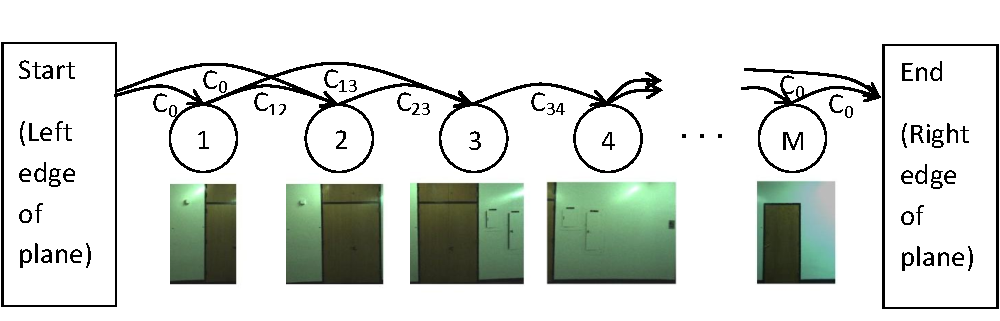
\includegraphics[width=3in]{dagCreation.pdf}
  \caption{DAG construction for the image selection process. \\}
  \label{fig:dagCreation}
\end{figure}

Figure \ref{fig:dagCreation} demonstrates the construction of a DAG
from overlapping images of a hallway wall. Images are sorted by
horizontal location left to right, and become nodes in a
graph. Directed edges are placed in the graph from left to right
between overlapping images. The weights of these edges are determined
by the SSD cost function. Next, we add two artificial nodes, one start
node representing the left border of the plane, and one end node
representing the right border of the plane. The left(right) artificial
node has directed edges with equal and arbitrary cost $C_0$ to(from)
all images that meet the left(right) border of the plane.

We now solve the shortest path problem from the start node to the end
node. This results in a set of images completely covering the plane
horizontally, while minimizing the cost of seams between images.

In rare cases where the vertical dimension of the plane is not
entirely covered by one or more chosen images, we are left with holes
where no images are selected to texture. Since these holes are rare,
and generally fairly small, we use a greedy approach, repeatedly
filling the hole with images that result in the lowest SSD costs in a
10 px border region around the hole. This method is not as optimal as
a true 2D-coverage solution would be, but it is a fast approximation,
and adequately handles the few holes we encounter.

With this completed, we have now mapped every location on the plane to
at least one image, and have minimized the number of images, as well
as the discontinuities at their borders. As seen in Figure
\ref{fig:compareAll}(d), this shortest path method has fewer visible
discontinuities than Figure \ref{fig:compareAll}(c) corresponding to
the tile caching approach\footnote{In Figure \ref{fig:compareAll}(d),
  we arbitrarily chose one image for texturing where images overlap,
  as blending will be discussed in section \ref{sec:blending}.}. This
is especially evident when comparing the posters in the images, which
have clear misalignment over seams in Figure \ref{fig:compareAll}(c),
but are much more aligned in Figure \ref{fig:compareAll}(d). This
shortest path approach approach directly reduces the cost of each
image boundary, while the tile caching method uses a scoring function
that only approximates this effect. Furthermore, seam minimization
guarantees the best selection of images, while the sequential tile
caching method may select images early on that turn out to be poor
choices once subsequent tiles have been processed. The seam
minimization approach is also far less intensive in terms of memory
usage and runtime, both during texture generation and rendering, as it
does not require discretizing planes or images.

When texturing an entire 3D planar model, we apply the seam
minimization approach on walls, due to its superior output when
provided with head-on images. Floors and ceilings however, given their
many images taken at oblique angles, are textured using the tile
caching method.


\subsection{Blending}
\label{sec:blending}
We now apply a blending procedure to both texturing methods. Although
the image alignment steps and image selection in both methods attempt
to minimize all mismatches between images, there are occasional
unavoidable discontinuities in the final texture due to different
lighting conditions or inaccuracies in planar geometry. These can
however be treated and smoothed over by applying alpha blending over
image seams.  Whether the units we are blending are
rectangularly-cropped images or rectangular tiles, we can apply the
same blending procedure, as long as we have a guaranteed overlap
between units to blend over.

For the tile caching method, we can ensure overlap by texturing a
larger tile than needed for display. For example, for a rendered tile
$l_1 \times l_1$, we can associate it with a texture $(l_1 + l_2)
\times (l_1 + l_2)$ in size.  We have found $l_2 = \frac{l_1}{2}$ to
provide a balance between blending and keeping features unblurred. For
the shortest path method, we have already ensured overlap between
images. To enforce consistent blending however, we add a minimum
required overlap distance of 40 px while solving the shortest path
problem in Section \ref{sec:shortestPath}. Additionally, if images
overlap in a region greater than the overlap distance, we only apply
blending over an area equal to the overlap distance.

After performing linear alpha blending across overlapping regions, our
texture mapping process is complete. Figures \ref{fig:compareAll}(e)
and \ref{fig:compareAll}(f) show the blended versions of Figures
\ref{fig:compareAll}(c) and \ref{fig:compareAll}(d) respectively. It
is clear that the shortest path approach exhibits better alignment and
fewer seams than the tile-caching method, as Figure
\ref{fig:compareAll}(f) has the best visual quality among the textures
in Figure \ref{fig:compareAll}.

\section{Results and Conclusions}
\label{sec:resultsAndConclusions}
Examples of ceilings and floors textured with the tile caching
approach, and walls textured with the shortest path approach, are
displayed in Figure \ref{fig:results}. High resolution texture
comparisons, as well as a walkthrough of a fully textured 3D model are
available in the accompanying video to this paper.

As mentioned earlier, our approach is fairly efficient, with the X by
X pixel image in figure X, spanning an X meter long wall and
consisting of X input images, taking under a minute to generate on a
2.8Ghz dual-core laptop, using the shortest path method. While not
fast enough for real-time visualization, the procedure is quick enough
for quick evaluation given changes in various internal parameters or
modifications to input data.

\subsection{Future stuff}
For the sake of simplicity, - cases where multiple whatever are few,
but for true generality, should go to 3d adjustments


\begin{figure*}
  \centering
  \subfloat[][]{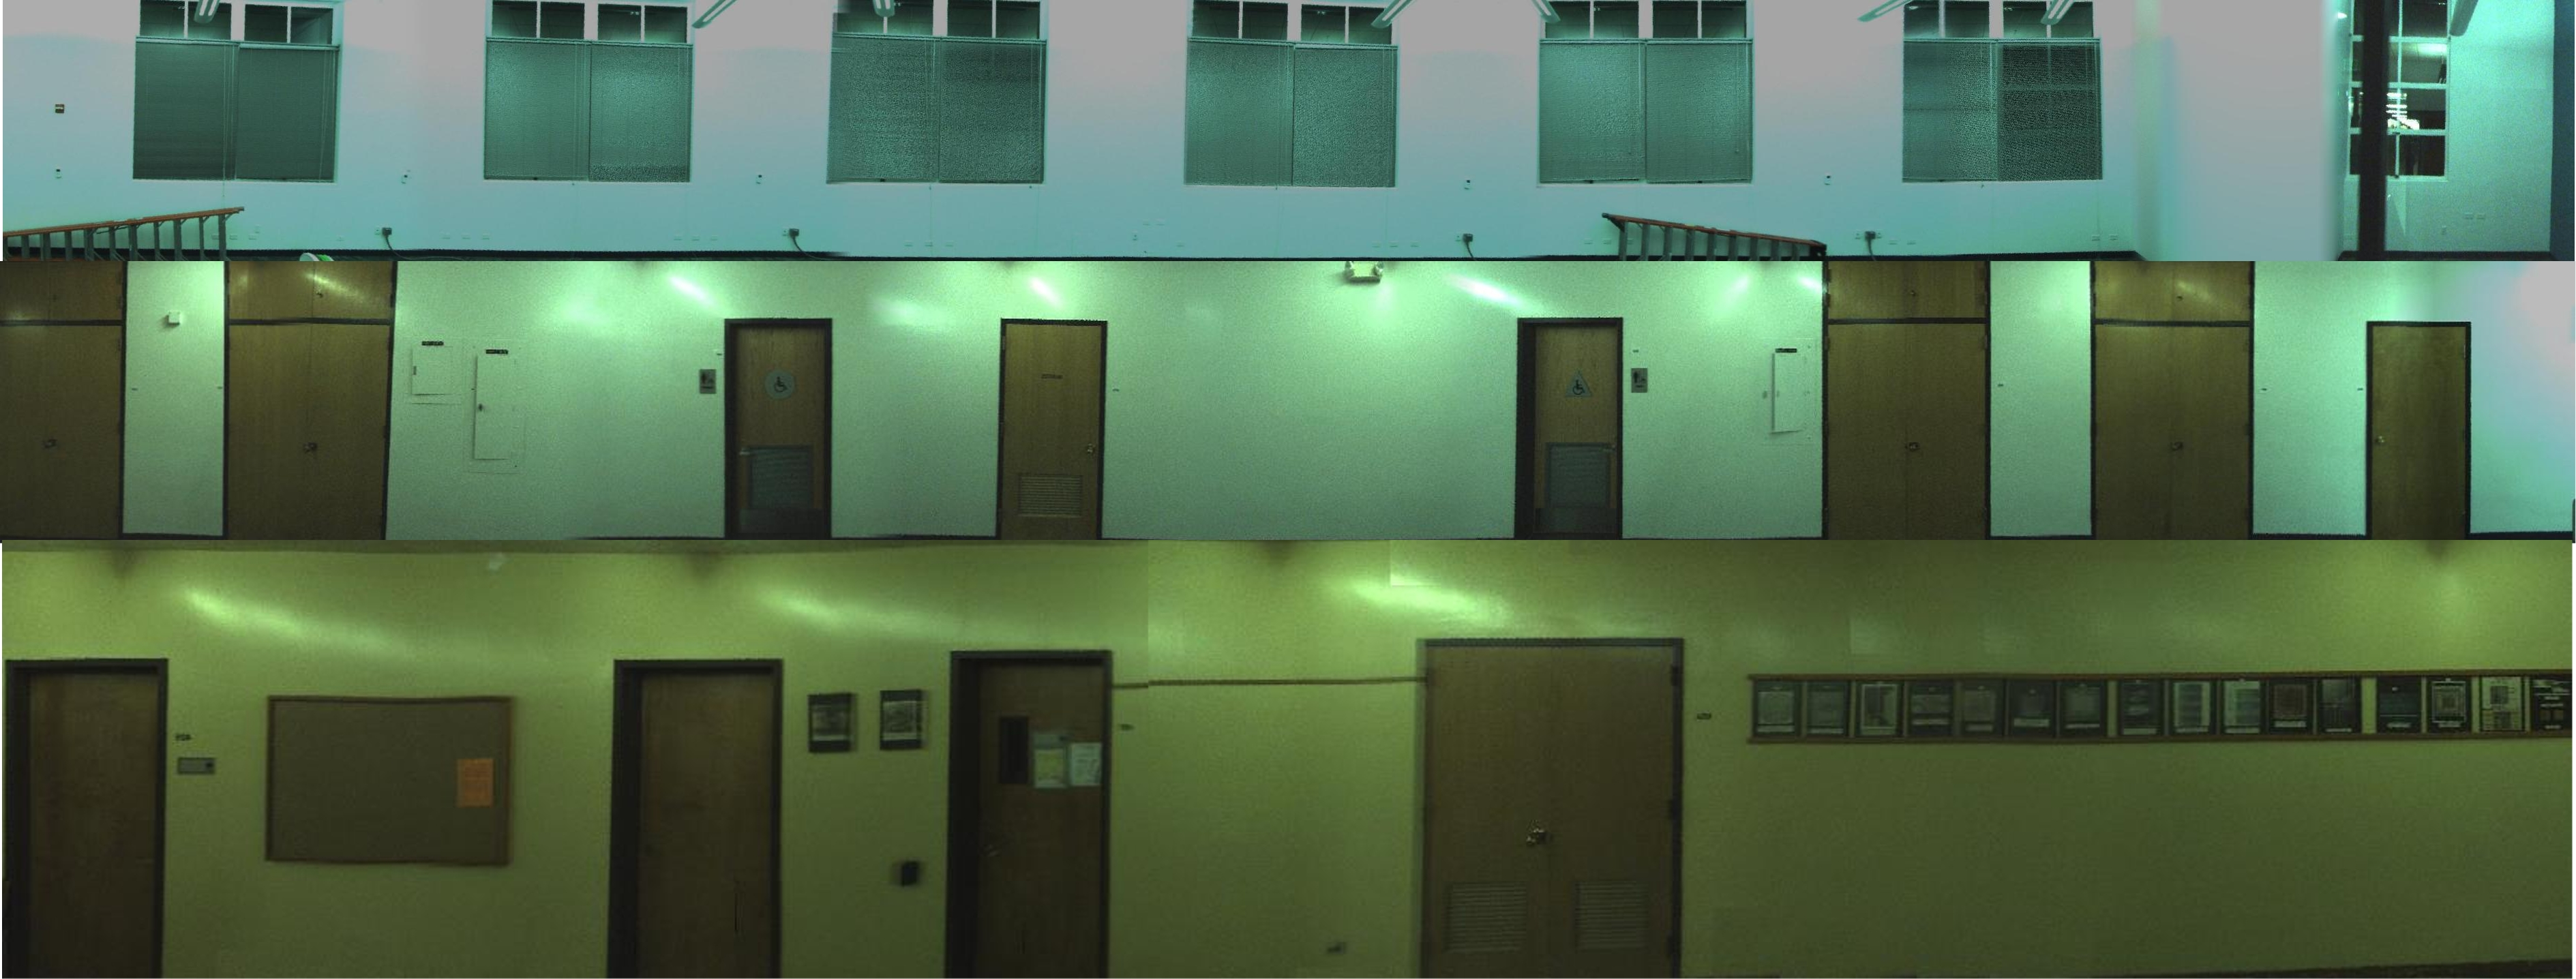
\includegraphics[width=3in]{finalfloors.jpg}}
  ~~~~~~~~
  \centering
  \subfloat[][]{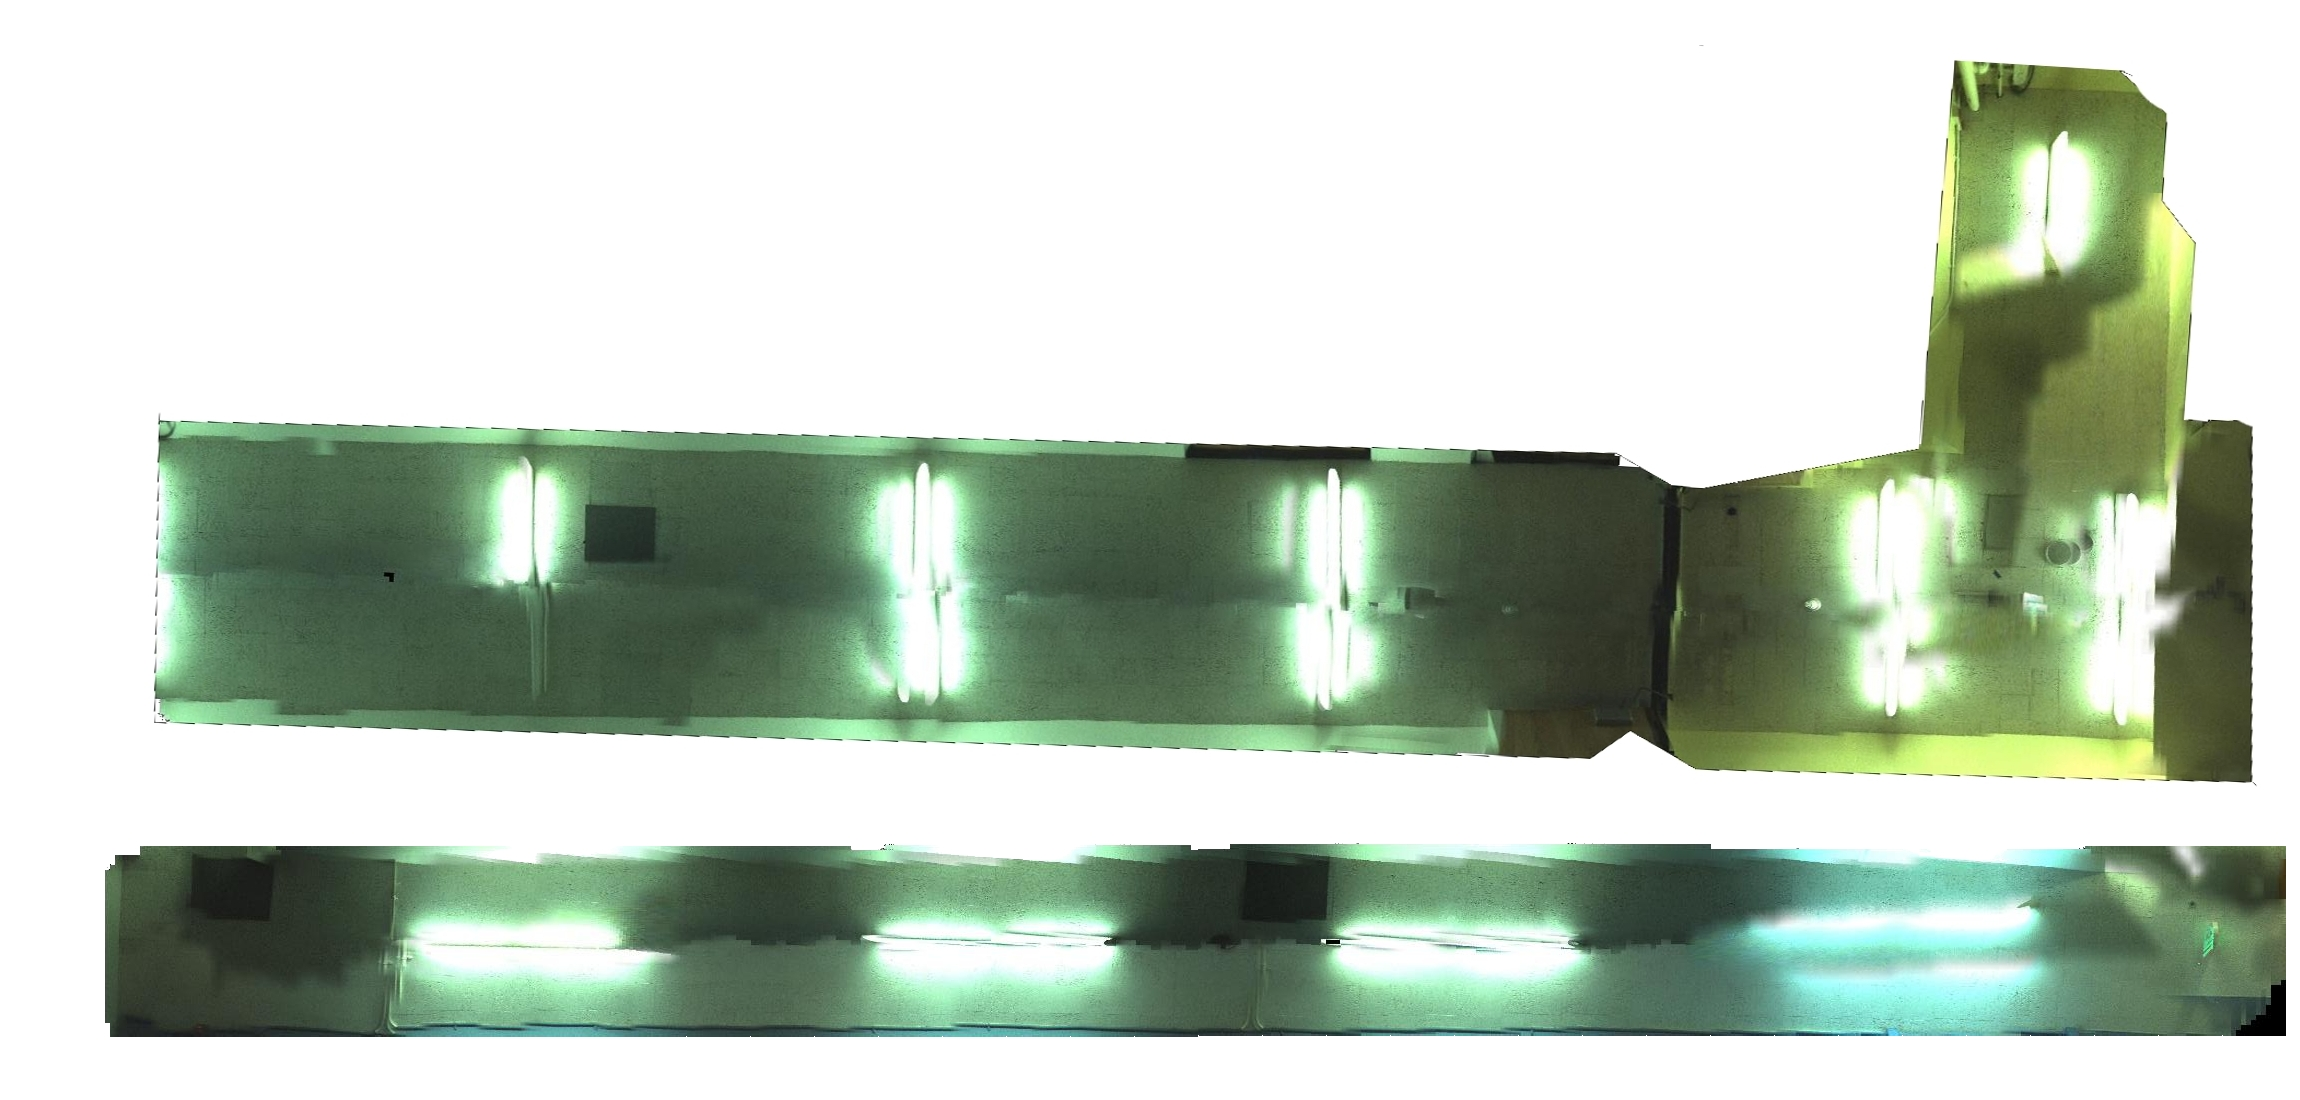
\includegraphics[width=3in]{finalceilings.jpg}}

  \centering 
  \subfloat[][]{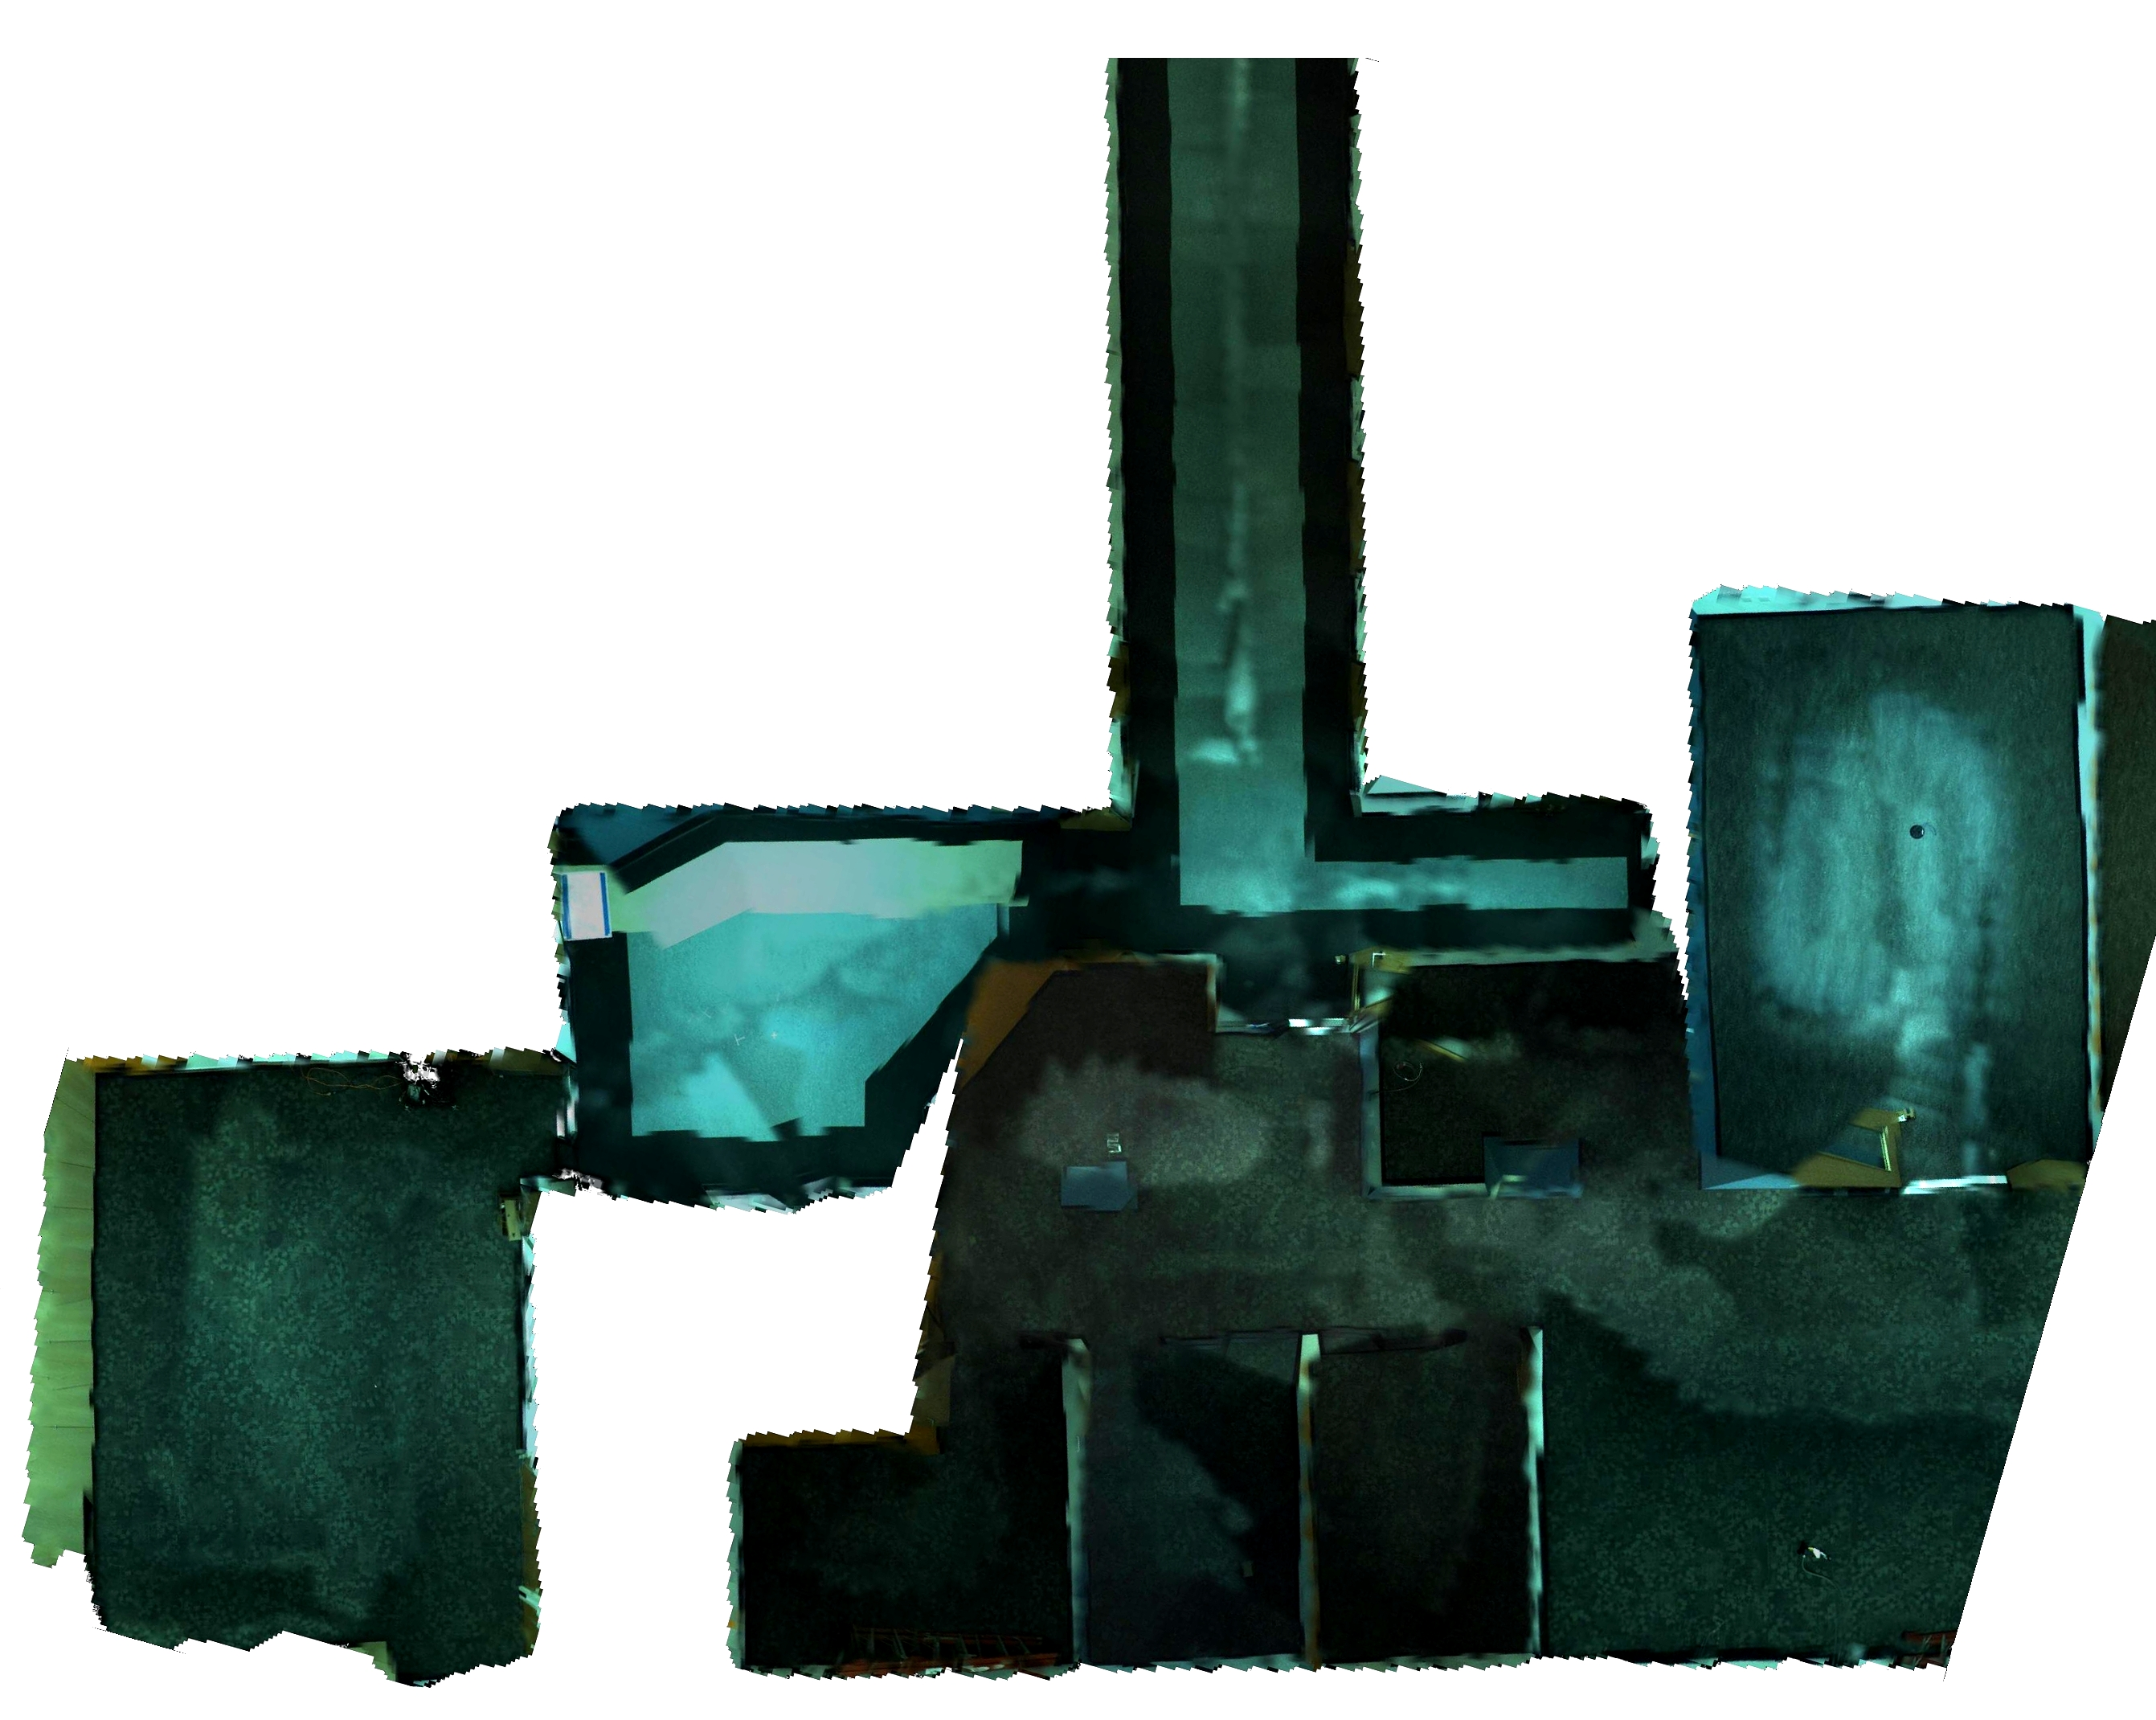
\includegraphics[height=2in, width=3in]{floorcropped.jpg}}
  ~~~~~~~~
  \centering
  \subfloat[][]{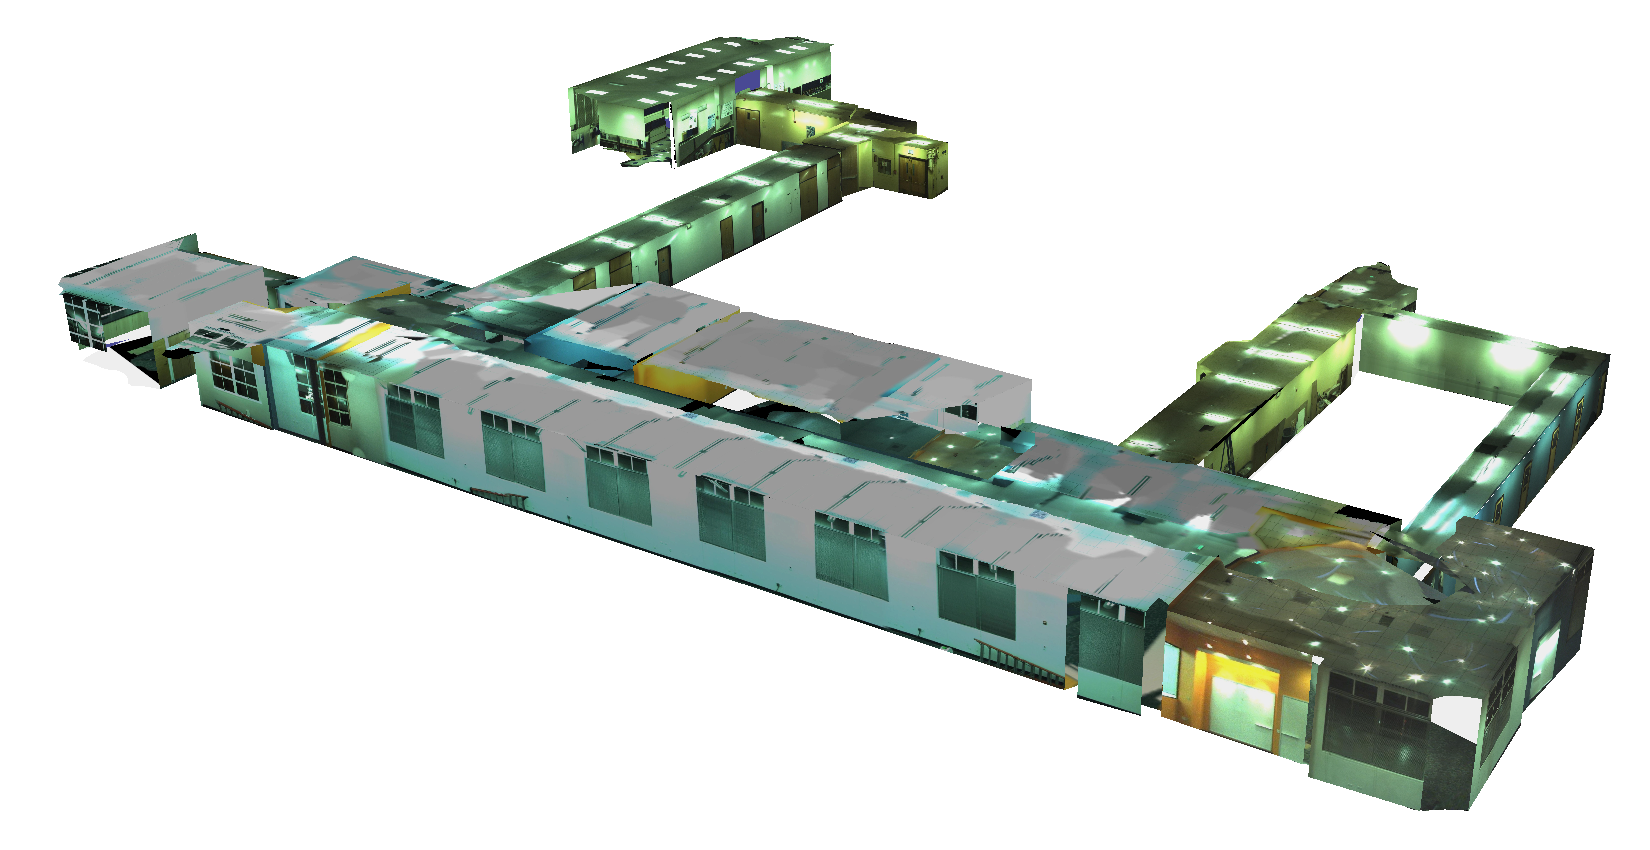
\includegraphics[width=3in]{fullmodel.png}}
  \caption{Examples of our final texture mapping output for (a) walls,
    (b) ceilings, (c) an entire floor, (d) a full model.}
  \label{fig:results}
\end{figure*}


%%%%%%%%%%%%%%%%%%%%%%%%%%%%%%%%%%%%%%%%%%%%%%%%%%%%%%%%%%%%%
%%%%% References %%%%%

\bibliography{report} %>>>> bibliography data in report.bib
\bibliographystyle{spiebib} %>>>> makes bibtex use spiebib.bst

\end{document} 
